\subsection{Almacenando tractogramas: Matrices ralas}
\label{sec:ralas}

Los m\'etodos para parcelar la corteza utilizados en este trabajo est\'an
basados en el $clustering$ de tractogramas. Podemos ver en la figura 
\ref{fig:diagrama} que primero generamos los tractogramas y luego se los
damos a un algoritmo para que los agrupe. Entre estos pasos es necesario
almacenar o mantener en memoria los tractogramas. En esta secci\'on
veremos como aprovechar la propiedad rala de los tractogramas para 
almacenarlos eficientemente. Tambi\'en mostramos como recuperar esta
propiedad luego de transformarlos al espacio $LogOdds$. \\ 
 
A modo de ejemplo situamos $762$ semillas en el \'area de Broca de un 
sujeto y generamos sus tractogramas. Aplanamos todos los tractogramas
a una sola dimensi\'on y los usamos como filas de una matriz. La matriz 
resultante tiene dimensiones $762\times3587328$. Asumiendo que cada valor
se representa usando $8$ Bytes ({\it double precision}), esta matriz ocupa
un total de
aproximadamente $20$ Gigabytes. Sin embargo, solo un $1\%$
de los datos almacenados son no nulos. Esto implica que casi todo el
espacio utilizado es desperdiciado.\\

\begin{figure}[h!]
   \centering
    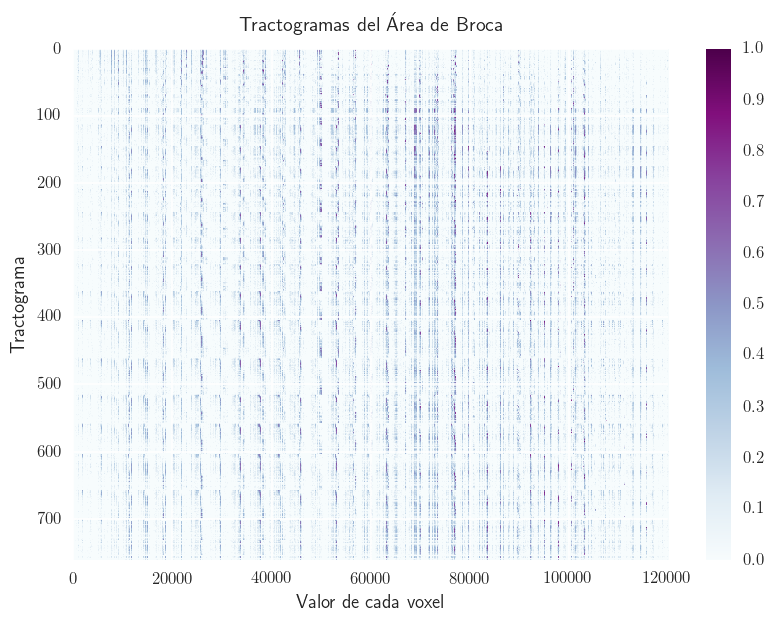
\includegraphics[width=0.9\textwidth]{img/densa_broca.png}
    \caption{Matriz con los tractogramas generados en el \'area de Broca
             de un sujeto. Las columnas cuyos valores eran todos nulos
             fueron removidas. }
    \label{fig:densa}
\end{figure}

Una forma de reducir el espacio requerido para almacenar la matriz es 
eliminar las columnas con solo elementos nulos. La figura \ref{fig:densa}
muestra la matriz que resulta de eliminar las columnas vac\'ias de la matriz
del \'area de Broca. Manteniendo la representaci\'on de $8$ Bytes este
proceso reduce el espacio necesario a aproximadamente $700$ Megabytes.
Si bien esto es una gran mejora, la nueva matriz posee solo un $27\%$ de
valores no nulos. Seguimos desperdiciando mucho espacio. \\

En el caso de crear los tractogramas de todo el hemisferio derecho usando
$21657$ semillas el eliminar columnas no es suficiente. La matriz
resultante posee dimensiones $21657\times3587328$. En esta, solo un $1\%$
de los valores son no nulos. Para almacenar dicha matriz es necesario
utilizar $587$ Gigabytes. Por esto es necesario utilizar estructuras mas
eficiente, que aprovechen lo ralo de las matrices. Ejemplos de estas
estructuras son: \textit{Dictionary of Keys}, o una matriz 
\textit{Compressed Sparse Row} (CSR). \\

%eliminando columnas in\'utiles nos queda 21657x145574, son 23.5 Gn

Al momento querer aplicar esto en nuestro m\'etodo nos encontramos con un
inconveniente. Nosotros transformamos los tractogramas al espacio $LogOdds$
antes de agruparlos. Por la forma que tiene la funci\'on $logit$ 
(ecuaci\'on \ref{eq:logit}) los tractogramas transformados ya no son ralos. 
Podemos ver en la figura \ref{fig:dominio} que 
\textit{logit}$(0) = -\infty$. Esto implica que la transformaci\'on de una
matriz rala no es rala en t\'erminos de elementos nulos. Sin embargo
podemos aprovechar ciertas propiedades para recuperar las matrices ralas.
La distancia euclidiana entre vectores es invariante a traslaciones lineales
del sistema. Lo mismo sucede con las posiciones relativas de los
$centroides$. Asignemos una representaci\'on finita $c$ al valor $-\infty$.
Un buen candidato para $c$ es el $log(\epsilon)$, donde $\epsilon$ es el
\textit{epsilon de la maquina}. Transformar todos los vectores y luego
trasladarlos sumando $c$ en cada componente dar\'a como resultado una
representaci\'on rala. Gracias a esto podemos utilizar DOK, CSR o cualquier
estructura para reducir el espacio necesario para almacenar los
tractogramas. \\

Dadas dos matrices ralas existen maneras eficientes de multiplicarlas entre
si \cite{Bank1993}. Si calculamos la distancia euclidiana entre dos vectores
ralos usando la siguiente relaci\'on: 

\begin{equation}
\label{eq:simileuc}
simil_{euc}(X,Y) = \sqrt{X \cdot X^t - 2 X \cdot Y^t + Y \cdot Y^t} 
\end{equation}

Podemos generar la matriz de distancias usando directamente las estructuras
de matrices ralas. Es importante destacar que este m\'etodo generara una
matriz que no necesariamente es sim\'etrica. Algunos valores que deber\'ian
ser iguales pueden presentar un peque\~no error num\'erico. Esto nos
permite utilizar matrices ralas durante todo el proceso de parcelamiento de
la corteza. \\


